% ****** Start of file apssamp.tex ******
%
%   This file is part of the APS files in the REVTeX 4.1 distribution.
%   Version 4.1r of REVTeX, August 2010
%
%   Copyright (c) 2009, 2010 The American Physical Society.
%
%   See the REVTeX 4 README file for restrictions and more information.
%
% TeX'ing this file requires that you have AMS-LaTeX 2.0 installed
% as well as the rest of the prerequisites for REVTeX 4.1
%
% See the REVTeX 4 README file
% It also requires running BibTeX. The commands are as follows:
%
%  1)  latex apssamp.tex
%  2)  bibtex apssamp
%  3)  latex apssamp.tex
%  4)  latex apssamp.tex
%
\documentclass[%
%reprint,
%superscriptaddress,
%groupedaddress,
%unsortedaddress,
%runinaddress,
%frontmatterverbose, 
preprint,
%showpacs,preprintnumbers,
%nofootinbib,
%nobibnotes,
%bibnotes,
 amsmath,amssymb,
 aps,
%pra,
%prb,
%rmp,
%prstab,
%prstper,
%floatfix,
]{revtex4-1}

\usepackage{graphicx}% Include figure files
\usepackage{dcolumn}% Align table columns on decimal point
\usepackage{bm}% bold math
%\usepackage{hyperref}% add hypertext capabilities
%\usepackage[mathlines]{lineno}% Enable numbering of text and display math
%\linenumbers\relax % Commence numbering lines

%\usepackage[showframe,%Uncomment any one of the following lines to test 
%%scale=0.7, marginratio={1:1, 2:3}, ignoreall,% default settings
%%text={7in,10in},centering,
%%margin=1.5in,
%%total={6.5in,8.75in}, top=1.2in, left=0.9in, includefoot,
%%height=10in,a5paper,hmargin={3cm,0.8in},
%]{geometry}


%%%%%%%%%%%%%%%%%%%%%%%%%%%
%%%%%%  PREAMBLES %%%%%%%%%
\newcommand{\ud}[1]{{#1^{\dagger}}}
\newcommand{\bra}[1]{\left\langle #1\right|}
\newcommand{\ket}[1]{\left| #1\right\rangle}
\newcommand\Tr{\mathrm{Tr}}
\newcommand{\braket}[2]{\langle #1 \mid #2 \rangle}
\newcommand\I{\mathbb{I}}
\newcommand{\avg}[1]{\left< #1 \right>}
\newcommand{\sech}[1]{{\operatorname{sech}{#1}}}
\newcommand{\csch}[1]{{\operatorname{csch}{#1}}}
%%%%%%  PREAMBLES %%%%%%%%%
%%%%%%%%%%%%%%%%%%%%%%%%%%%

\begin{document}

%\preprint{APS/123-QED}

\title{Neutrino Oscillations - A Rabi Oscillation View}% Force line breaks with \\
%\thanks{A footnote to the article title}%

\author{Lei Ma}
\email{leima@unm.edu}
\author{Shashank Shalgar}%
\email{shashankshalgar@unm.edu}
\author{Huaiyu Duan}%
\email{duan@unm.edu}
\affiliation{%
 Department of Physics \& Astronomy, University of New Mexico,
 Albuquerque, NM 87131, USA
}%
% \author{Huaiyu Duan}%
%  \email{Second.Author@institution.edu}
% \affiliation{%
%  Authors' institution and/or address\\
%  This line break forced with \textbackslash\textbackslash
% }%

% \collaboration{MUSO Collaboration}%\noaffiliation

% \author{Shashank Shalgar}
%  \homepage{http://www.Second.institution.edu/~Charlie.Author}
% \affiliation{
%  Second institution and/or address\\
%  This line break forced% with \\
% }%
% \affiliation{
%  Third institution, the second for Charlie Author
% }%
% \author{Delta Author}
% \affiliation{%
%  Authors' institution and/or address\\
%  This line break forced with \textbackslash\textbackslash
% }%

% \collaboration{CLEO Collaboration}%\noaffiliation

% \author{Huaiyu Duan}
%  \homepage{http://www.Second.institution.edu/~Charlie.Author}
% \affiliation{
%  Second institution and/or address\\
%  This line break forced% with \\
% }%
% \affiliation{
%  Third institution, the second for Charlie Author
% }%
% \author{Delta Author}
% \affiliation{%
%  Authors' institution and/or address\\
%  This line break forced with \textbackslash\textbackslash
% }%

% \collaboration{CLEO Collaboration}%\noaffiliation



\date{\today}% It is always \today, today,
             %  but any date may be explicitly specified

\begin{abstract}
ABSTRACT PLACEHOLDER
% \begin{description}
% \item[Usage]
% Secondary publications and information retrieval purposes.
% \item[PACS numbers]
% May be entered using the \verb+\pacs{#1}+ command.
% \item[Structure]
% You may use the \texttt{description} environment to structure your abstract;
% use the optional argument of the \verb+\item+ command to give the category of each item. 
% \end{description}
\end{abstract}

% \pacs{Valid PACS appear here}% PACS, the Physics and Astronomy
                             % Classification Scheme.
%\keywords{Suggested keywords}%Use showkeys class option if keyword
                              %display desired
\maketitle

%\tableofcontents

\section{\label{introduction}Introduction}

In many astrophysical environments neutrinos propagate through dense fluctuating medium, which will interact with neutrinos and dramatically change the flavor oscillations of neutrinos. The significance of matter effect on neutrino flavor oscillations has been demonstrated in Mikheyev–Smirnov–Wolfenstein effect (MSW effect), which plays a role in solar neutrino oscillations.\cite{wolf78} Another matter effect of interest is parametric resonance of neutrino flavor oscillations due to perturbations in matter.\cite{Krastev1989} Recently matter stimulated neutrino oscillations has been researched using more advanced mathematical tools by Kneller, et al..\cite{Kneller2013,Patton2014} They have shown that many stimulated neutrino oscillations can be explained by resonances of the system. 

In this manuscript, we take a step further and interpret matter effect, both MSW resonance and parametric resonance, as superposition of Rabi oscillations. Using a specific unitary transformations of the states, we can rewrite the system into a superposition of Rabi oscillations and investigate the resonances of each mode.



\section{\label{rabi}Neutrino Oscillations in Matter and Rabi Oscillation}%


%% Introduction to neutrino oscillations in matter




In this section we present the relation between neutrino oscillations in matter and Rabi oscillation using a system with single frequency perturbations in the matter profile $\lambda(x)\equiv\sqrt{2}G_{\mathrm F} n_{\mathrm e}(x)$, which is specifically written as
\begin{equation}
    \lambda(x) = \lambda_0 + A \sin (k x) ,
\end{equation}
where $G_{\mathrm F}$ is the Fermi constant and $n_{\mathrm e}(x)$ is the electron number density in the medium. For better understanding of the transition between states, we use the background matter basis, in which the Hamiltonian is diagonalized in the absence of perturbation $A\sin(kx)$, so that the Hamiltonian becomes
\begin{equation}
    H^{(\mathrm{m})} = -\frac{\omega_3}{2} \sigma_3 + \frac{1}{2} A\sin (kx) \cos 2\theta_{\mathrm m} \sigma_3 -\frac{1}{2} \sin(kx) \sin 2\theta_{\mathrm m} \sigma_1,\label{neutrino-matter-single-frequency-hamiltonian}
\end{equation}
where $\sigma_i$ are the Pauli matrices, $\theta_{\mathrm m}$ is the mixing angle in a constant matter profile $\lambda_0$, which is calculated using relation $\tan 2\theta_{\mathrm{m}}=\sin 2\theta_{\mathrm v}/\left( \cos 2\theta_{\mathrm v} - \lambda_0/\omega_{\mathrm v} \right)$ with $\omega_{\mathrm v}$ denoting the vacuum oscillation frequency and $\theta_{\mathrm v}$ denoting the vacuum mixing angle.

To make connections with Rabi oscillation, we argue that the second term in Hamiltonian is not relevant when the system is close to resonance. FIG.~\ref{fig-rabi-oscillations-energy-gap-change} \verb|+| marker shows transition probability of neutrino oscillation in matter.




%%%%%%%%%
%%%%%%%%% Rabi oscillation
%%%%%%%%%

\subsection{Rabi Oscillation}


An optical field interacts with two-level atoms and can stimulate transition from low energy state to high energy state. As the frequency of optical field approaches the energy split of atom, large transition occurs, which is described by Rabi oscillation. Rabi oscillation has been well studied in quantum optics.\cite{Boyd2008} 

The Hamiltonian we use as an example is
\begin{equation}
    H_{\mathrm R} = - \frac{\omega_{\mathrm m}}{2} - \frac{1}{2}A_{1} \cos (k_1 x) \sigma_1 + \frac{1}{2} \sin (k_1 x) \sigma_2,\label{rabi-oscillation-single-perturbation}
\end{equation}
in which $\omega_{\mathrm m}$ serves as the energy split of the two level system, while $A_1$ and $k_1$ are the strength and frequency of the driving field, respectively. Such a system has analytical transition probability from low energy state to high energy state
\begin{equation}
    P(x) = \frac{\left \lvert A_1 \right \rvert ^2}{ \Omega_{\mathrm R}^2 } \sin^2 \left( \frac{\Omega_{\mathrm R}}{2} x \right),
\end{equation}
where $\Omega_{\mathrm R} = \sqrt{ \lvert A_1\rvert^2 + (k_1 - \omega_{\mathrm m})^2 }$ is known as Rabi frequency. The detuning, which is defined as $k_1 - \omega_{\mathrm m}$, determines how off-resonance the system is, and amplitude of optical field $A_1$ determines the resonance width. The transition probability oscillates with frequency $\Omega_{\mathrm R}$, however, optical field amplitude $A_1$ is the dominate factor for oscillation frequency when the system is close to resonance.






To show that neutrino oscillations can be treated as Rabi oscillations, we calculate transition probabilities of the neutrinos described by Eq.~(\ref{neutrino-matter-single-frequency-hamiltonian}), and the Rabi oscillations described by Eq.~(\ref{rabi-oscillation-single-perturbation}), with parameters chosen so that the two systems have the same energy split and driving field strength and frequency. The \verb|+| marker is the result of neutrino oscillations, meanwhile we display the result of Rabi oscillation using $\circ$ in FIG.~\ref{fig-rabi-oscillations-energy-gap-change}.

\fbox{
\parbox{0.9\textwidth}{\bf Maybe a plot that shows the comparison of the predicted amplitudes and numerical amplitudes for different $A_2$'s.}
}


\begin{figure}[!htbp]
                \centering
                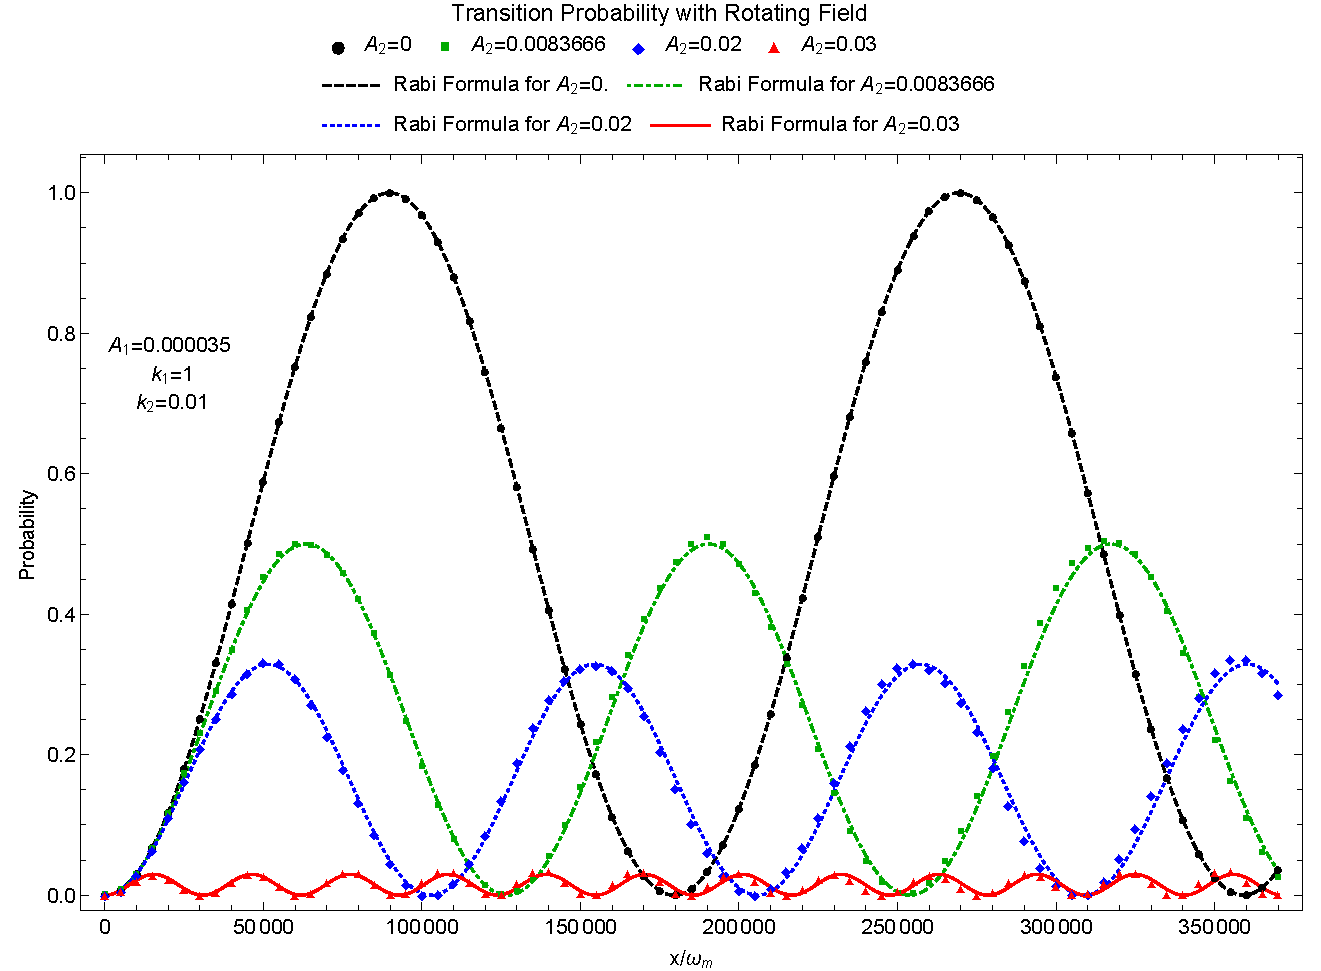
\includegraphics[width=\textwidth]{assets/rabi-oscillations-energy-gap-change-k2-0-01}
                \caption{Reduction of transition amplitudes. Black dashed line: the system has only one perturbation which is at exact resonance; Green dash-dotted line: $A_2=A_{2,\mathrm{Critical}}=0.0083666\omega_{\mathrm m}$; Blue dotted line: $A_2=0.01\omega_{\mathrm m}$; Red line: $A_2=0.02\omega_{\mathrm m}$. The markers are the probabilities predicted using Rabi formula correspondingly. Black cross is the transition probability between two background mass eigenstates for the neutrinos with matter perturbation $A\sin(kx)$.}
                \label{fig-rabi-oscillations-energy-gap-change}
\end{figure}



\subsection{Parametric Resonance}

The parametric resonance condition is exactly the condition of Rabi oscillations.







%%%%%%%%%%%%%%%%%%%%%%%%%%%%%%%%%%%%%%%%%%%%%%%%%%%%
%%%%%%%%%  Stimulated Neutrino Oscillations  %%%%%%%%%%%%%%%%%%%
%%%%%%%%%%%%%%%%%%%%%%%%%%%%%%%%%%%%%%%%%%%%%%%%%%%%

\section{\label{stimulated}Analysis of Stimulated Neutrino Oscillations Using Rabi Oscillations}



\subsection{Neutrino oscillations in matter}



\subsection{To Make connections to Rabi oscillation}



\subsubsection{Jacobi-Anger Expansion: Write the system into a superposition of Rabi oscillations.}
    
    




    

\subsection{The Important Factors}



\begin{itemize}
            \item Width of resonance $B$
            \item Deviation from exact resonance $g$, called {\bf{detuning}} (value).
            \item Oscillation wavelength of mode (determined by Rabi frequency, which is in turn related to $B$ and $g$ ) compared to size of physical system
\end{itemize}







\section{\label{conclusions}Conclusions}

%%%% Do not repeat what has been said

CONCLUSION PLACEHOLDER




\bibliographystyle{abbrv}
\bibliography{ref.bib} 



%%%%%%%%%%%%%%%%%%%%%%%%%%%%%%%%%%%%%%%%%%
%%%%%%%%%%%%% APPENDIX  %%%%%%%%%%%%%%%%%%
%%%%%%%%%%%%%%%%%%%%%%%%%%%%%%%%%%%%%%%%%%









\end{document}